\documentclass[12pt, oneside]{article}
\usepackage[T1]{fontenc}
\usepackage[spanish, es-tabla, es-lcroman]{babel}
\usepackage[utf8]{inputenc}
\usepackage[document]{ragged2e}
\usepackage{tcolorbox}
\tcbuselibrary{theorems}
\usepackage{cancel}
\usepackage{amssymb}
\usepackage{amsmath}
\usepackage{mathrsfs}
\usepackage{wrapfig}
\usepackage{fancyhdr}
\usepackage{colortbl}
\usepackage{longtable}
\usepackage{diagbox}
\usepackage{graphicx}
\usepackage{subcaption}
\usepackage{xcolor}
\usepackage{tikz}
\usetikzlibrary{positioning}
\usepackage{multicol}
\usepackage{multirow}
\usepackage{lastpage}
\usepackage{pdfpages}
\usepackage{listings}
\usepackage{blindtext}
\spanishdecimal{.}
\usepackage[explicit]{titlesec}
\usepackage[colorlinks=true, linkcolor=black, citecolor=black, urlcolor=blue]{hyperref}
\usepackage[a4paper, total={16cm, 24cm}]{geometry}
\pagestyle{fancy}
\lhead{Muñoz Nuñez Ian Emmanuel}
\rhead{Proyecto 10}
\lfoot{Mtra. María Patricia Ventura Nuñez}
\rfoot{CUCEI}
\renewcommand{\headrulewidth}{1pt}
\renewcommand{\footrulewidth}{1pt}

\setlength{\headheight}{14.49998pt}

\begin{document}

\begin{titlepage}
    \pagenumbering{roman}
    \centering
    {\bfseries\LARGE Universidad de Guadalajara \par}
    \vfill
    {
        \includegraphics[width=0.3\linewidth]{UdG.png}
        \includegraphics[width=0.3\linewidth]{qci.png}
        \par
    }
    \vfill
    {\bfseries\LARGE Seminario de programación de sistemas reconfigurables \par}
    \vfill
    {\ttfamily\LARGE Contadores en cascada \par}
    \vfill
    {\bfseries\LARGE Nombre: \par}
    \vfill
    {\bfseries\LARGE  Muñoz Nuñez Ian Emmanuel \par}
    \vfill
    {\bfseries\LARGE Sección: D01 \par}
    \vfill
    {\bfseries\LARGE Código: 216464457 \par}
    \vfill
    {\bfseries\LARGE Maestra: \par}
    \vfill
    {\bfseries\LARGE María Patricia Ventura Nuñez \par}
    \vfill
    {\bfseries\LARGE Ingeniería Robótica \par}
\end{titlepage}

\pagenumbering{arabic}

\newpage
\section{Objetivo}
{\sffamily\large
    \hspace{0.5cm} Solucionar problemas de diseño utilizando las herramientas aprendidas en
    programación de sistemas reconfigurables.

    \hspace{0.5cm} Simular circuitos digitales en progrmas de diseño como
    \emph{Proteus\textregistered} e implementarlos físicamente.

}

\section{Material}
{\sffamily\large
    \renewcommand{\labelitemi}{$\bullet$}
    \begin{itemize}
        \item Protoboard.
        \item Fuente VCC (5V).
        \item Resistencias $220\Omega$ y $2K\Omega$.
        \item Dip-switch de 8 y 4 bits.
        \item 2 contadores \emph{4029}.
        \item 2 decodificadores \emph{74LS48}.
        \item 1 compuerta \emph{AND}.
        \item 2 Display's de 7 segmentos de cátodo común.
    \end{itemize}

}

\section{Marco teórico}
{\sffamily\large
    \hspace{0.5cm} Para este proyecto lo más complicado fue entender el funcionamiento de los
    contadores, pero después de eso, es sencillo, pues cada que un contador termina su secuencia
    o se desborda, se manda la señal al siguiente contador, por lo que simplemente se tiene que
    conectar el el acarreo de salida (en el caso del contador \emph{4029}) o a la terminal de
    salida del conteo ascendente o descendente (en el caso del contador \emph{74LS193}).

}

\newpage
\section{Procedimiento}
{\sffamily\large
    \hspace{0.5cm} Para realizar el proyecto primero se entendió el funcionamiento de los
    contadores, una vez hecho eso, solo se conectaron los pines de \emph{preset} se conectaron
    correctamente para que la secuencia iniciara en $68$, que es el número con el que inicia mi
    secuencia en el circuito binario, y ya que en el circuito de \emph{BCD} la secuencia inicia
    en $0$, todas las entradas de \emph{preset} se conectaron a tierra. Las salidas se conectaron
    a los \emph{led's} en el caso del circuito en binario, y en el de \emph{BCD} se conectaron a
    los decodificadores, y la salida de estos se conecto a los \emph{display's}. Al final, se
    condicionaron las salidas de los contadores, para que cuando lleguen al último número de la
    secuencia estos se reiniciaran y así, la secuencia comenzara de nuevo.

    \hspace{0.5cm} Los materiales utilizados son: 1 dip-switch de 8 bits y otro de 4 bits,
    resistencias de $2k\Omega$ y de $220\Omega$, 12 \emph{led's}, 4 compuertas AND \emph{74LS08},
    2 decodificadores \emph{74LS48}, 2 \emph{display's} de 7 segmentos de cátodo común, y por
    último, 2 contadores \emph{4029} y 2 \emph{74LS193}.

}

\section{Circuito a implementar}
{\sffamily\large
    \hspace{0.5cm} El circuito que se eligió para implementar en protoboard fue el \emph{BCD},
    pues es más sencillo y visualmente más interesante.

}

\subsection{Simulación}
{\sffamily\large
    \hspace{0.5cm} En las siguientes 2 páginas se muestra el diseño de los circuitos en simulación.
    El primero es el circuito en binario, y el segundo en \emph{BCD}.

    \newpage
    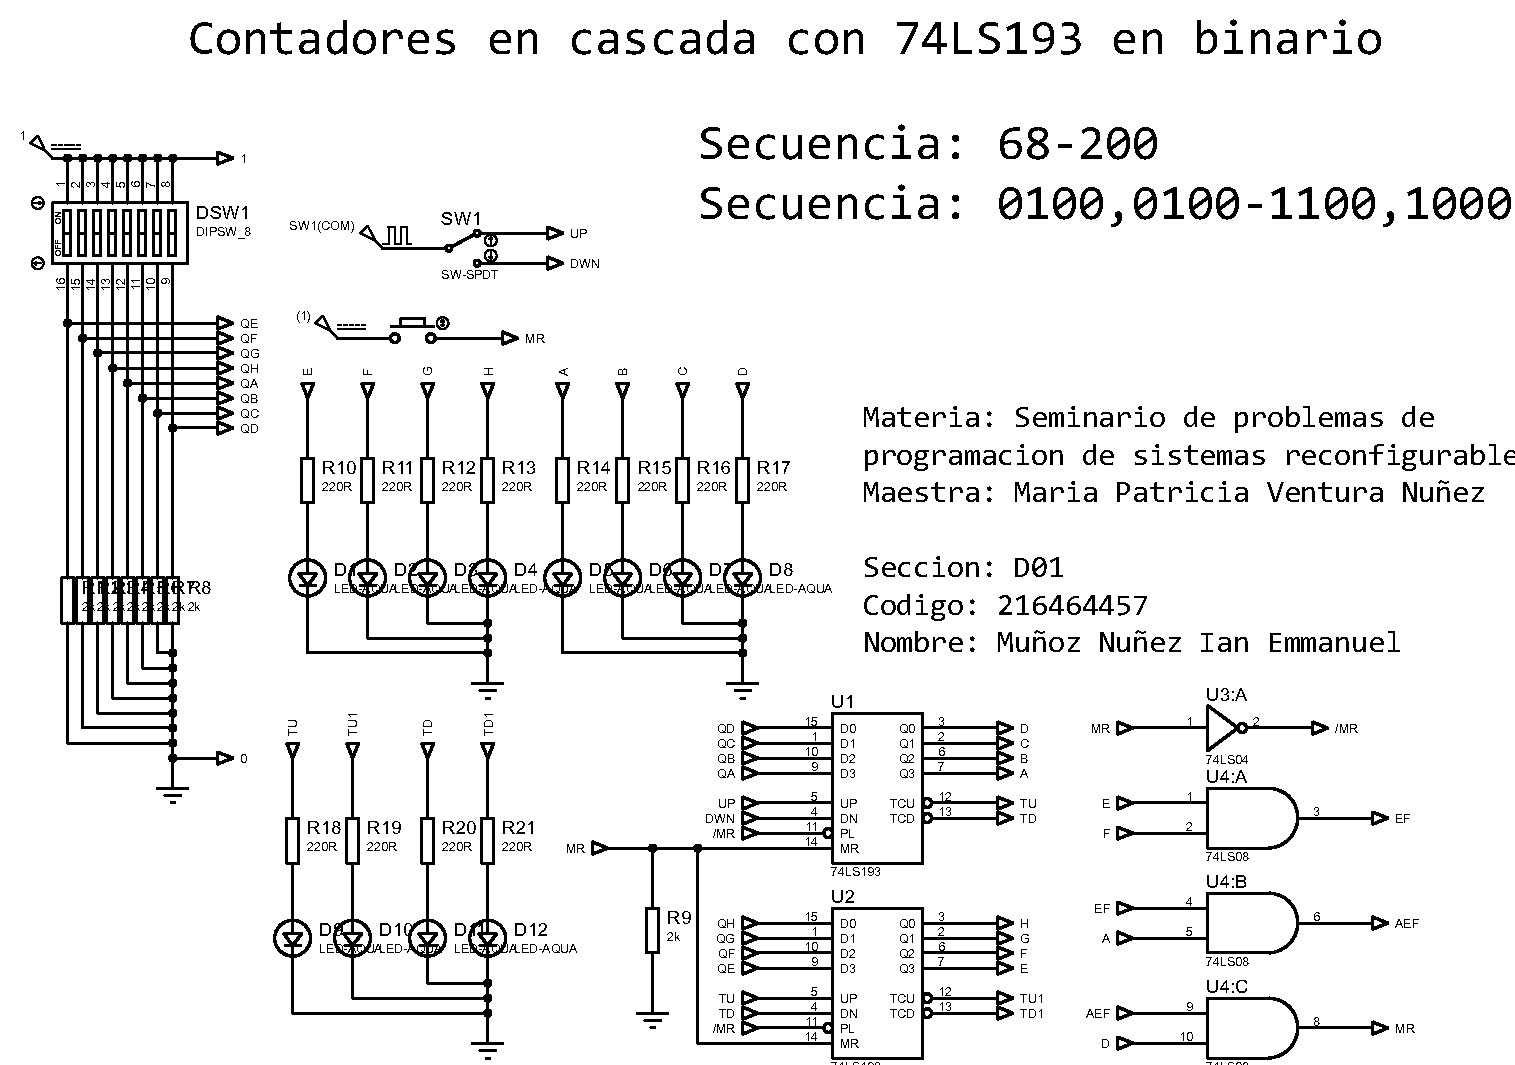
\includepdf[pages={1}]{main_binario_munozNunezIan.PDF}

    \newpage
    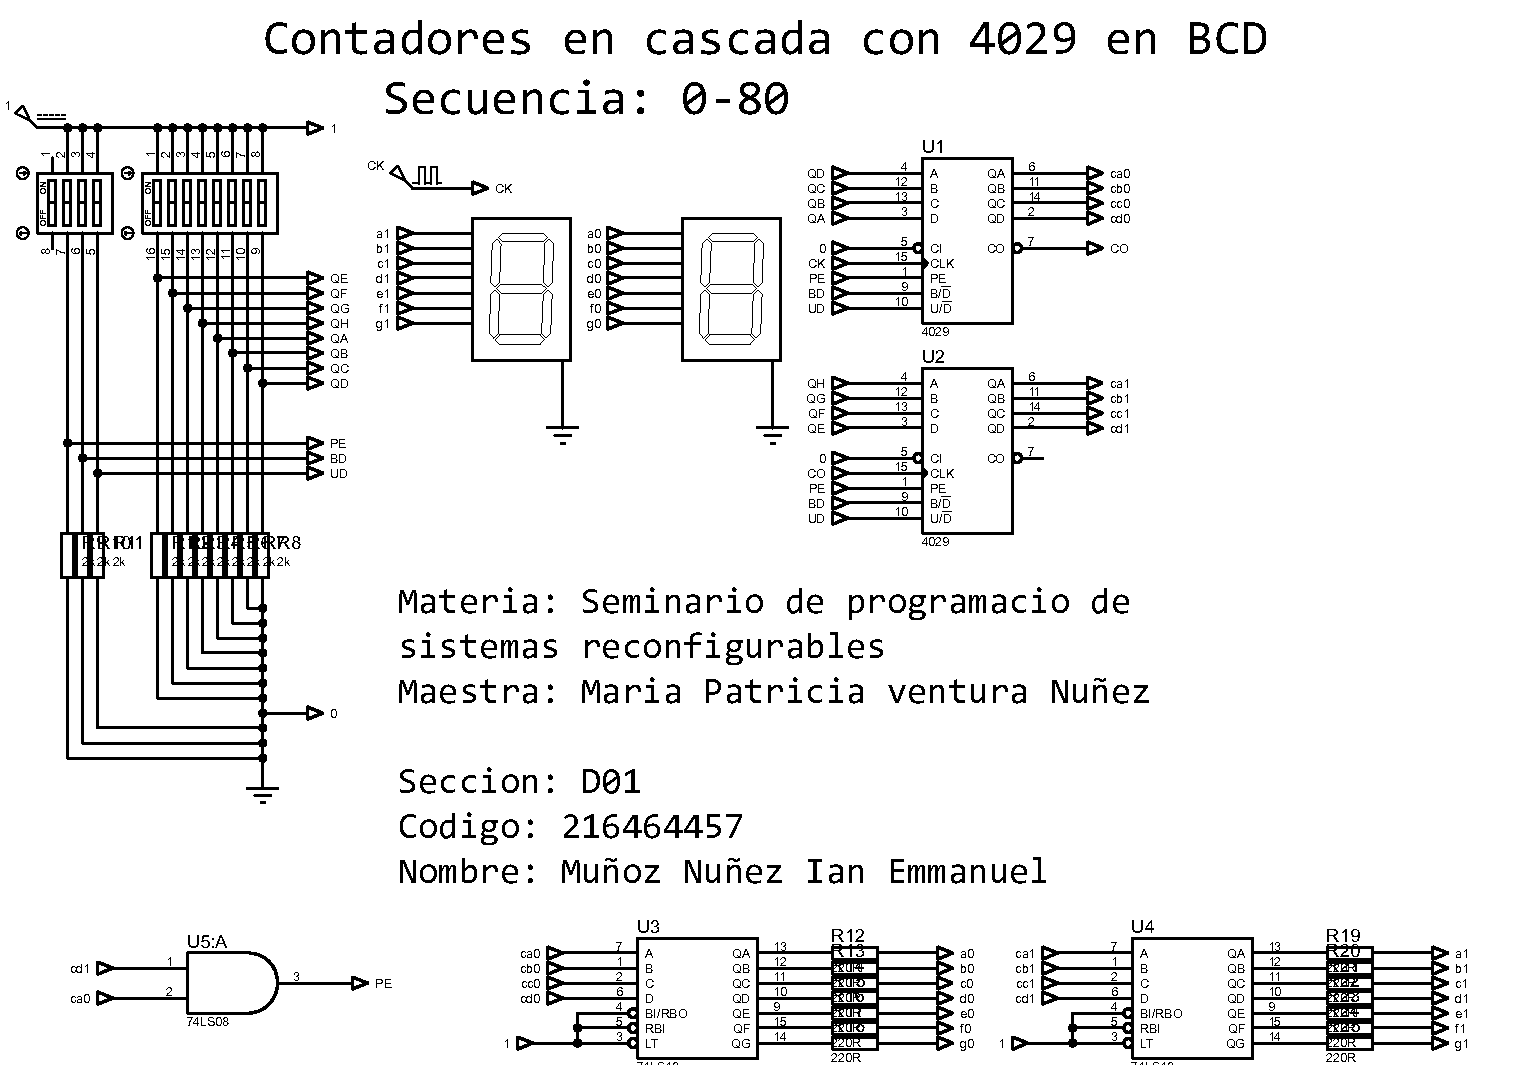
\includepdf[pages={1}]{main_bcd_munozNunezIan.PDF}

}

\newpage
\subsection{Protoboard}
\begin{figure}[h!]
    \centering

    \begin{subfigure}{0.45\textwidth}
        \centering
        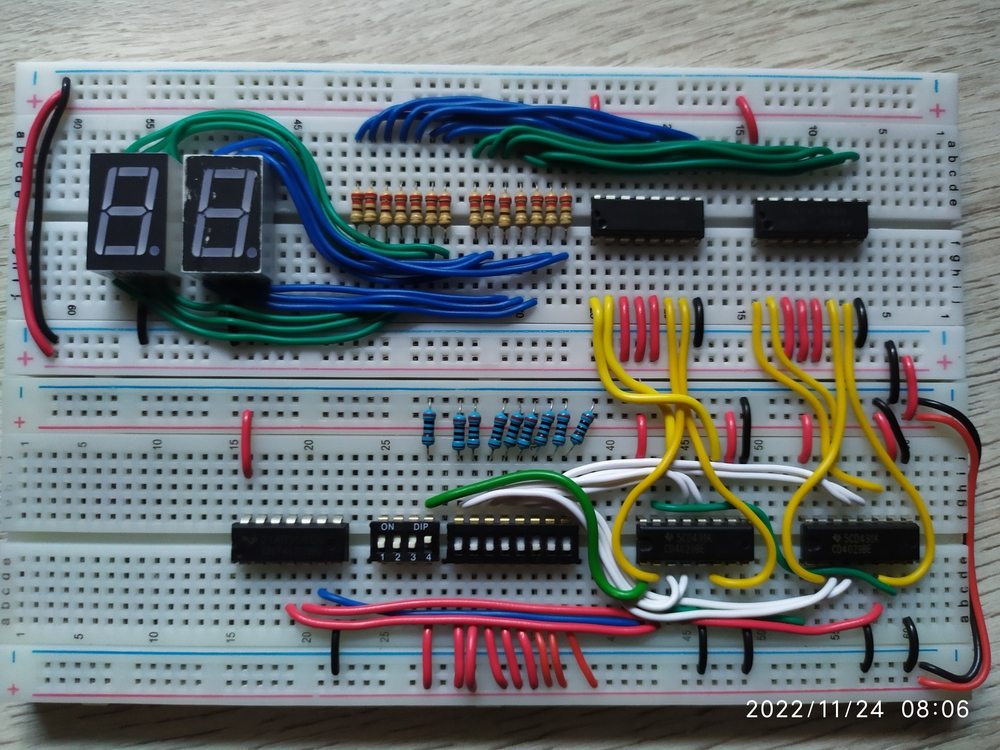
\includegraphics[width=\linewidth]{figs/IMG_20221124_080652.jpg}
    \end{subfigure}
    \begin{subfigure}{0.45\textwidth}
        \centering
        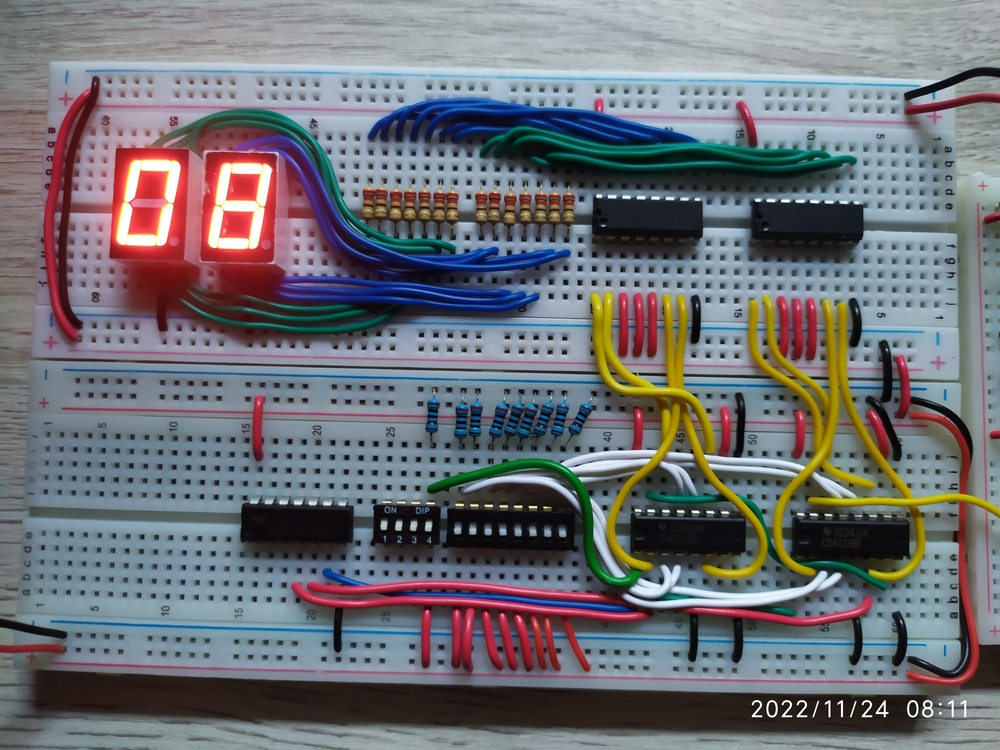
\includegraphics[width=\linewidth]{figs/IMG_20221124_081134.jpg}
    \end{subfigure}
    \begin{subfigure}{0.45\textwidth}
        \centering
        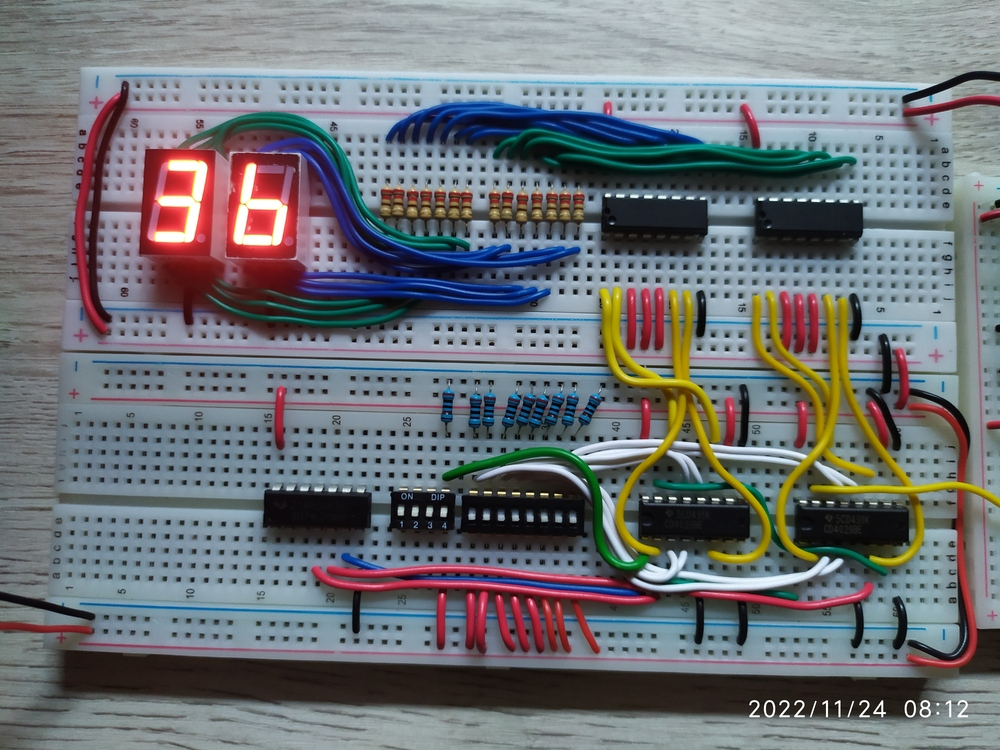
\includegraphics[width=\linewidth]{figs/IMG_20221124_081216.jpg}
    \end{subfigure}
    \begin{subfigure}{0.45\textwidth}
        \centering
        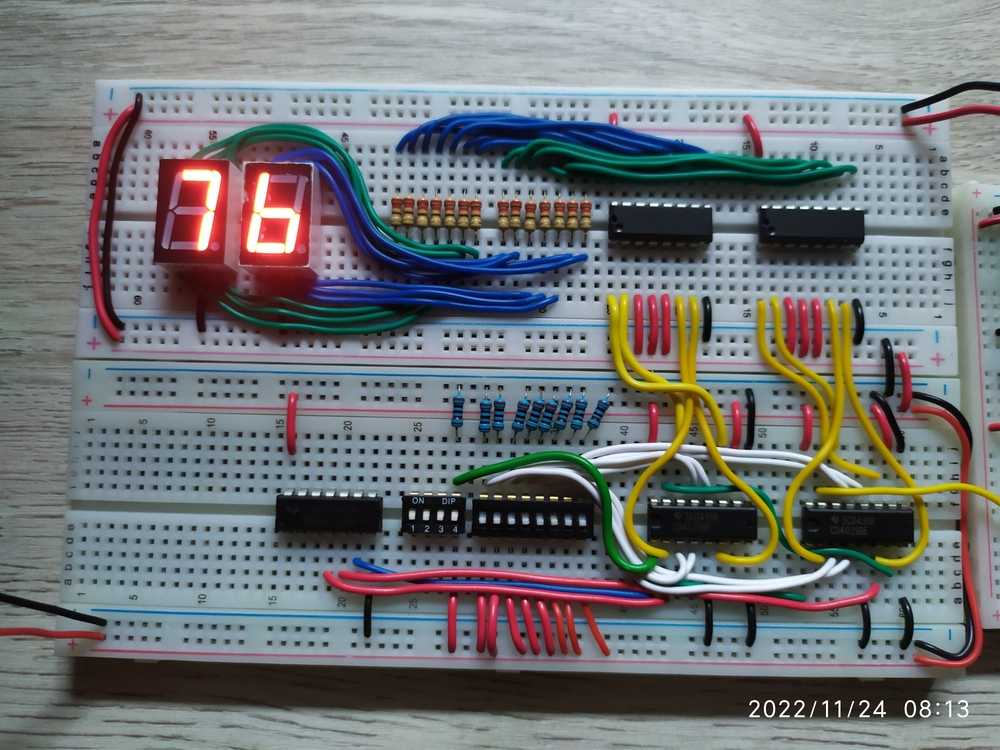
\includegraphics[width=\linewidth]{figs/IMG_20221124_081316.jpg}
    \end{subfigure}

    \caption{\sffamily Circuito en protoboard}
    \label{fig:proto}
\end{figure}

\section{Conclusión}
{\sffamily\large
    \hspace{0.5cm} Comprender el funcionamiento de los contadores es importante pues son
    componentes muy utilizados en los circuitos, y no de esta forma no es necesario diseñar por
    nuestra cuenta un contador, y tienen lo necesario para poder utilizarlos en bastantes
    escenarios, y lo mejor es que son baratos, accesibles y sencillos de comprender y usar.

}

\end{document}

